% ============================================================================
% Neuron-Level Structural Control Impact Reveals Visual-Centrifugal
% Chokepoints in the Drosophila Connectome
%
% Compile: pdflatex manuscript && bibtex manuscript && pdflatex manuscript &&
%          pdflatex manuscript
% Requires: article class + graphicx, amsmath, booktabs, geometry, hyperref
%           (a standard TeX Live / MiKTeX installation). Figures are vector
%           PDFs in figures/; tables are \input from tables/.
% The companion inspection PDF (manuscript_production.pdf) is rendered from
% manuscript_production.html via Edge headless for environments without a
% TeX toolchain; the .tex source above is the submission-grade source.
% ============================================================================
\documentclass[11pt]{article}
\usepackage[margin=1in]{geometry}
\usepackage{graphicx}
\usepackage{amsmath}
\usepackage{booktabs}
\usepackage[hidelinks]{hyperref}
\usepackage{microtype}

\graphicspath{{figures/}}
\title{\textbf{Neuron-Level Structural Control Impact Reveals\\
Visual-Centrifugal Chokepoints in the \emph{Drosophila} Connectome}}
\author{FAFB v783 Connectome Control-Impact Study\\
\small Frozen scientific results: E06--E14 (2026-09-15), E10B 100-null
confirmation (2026-09-17)}
\date{September 18, 2026}

\begin{document}
\maketitle

% Abstract
\begin{abstract}
\noindent\textbf{Background.} The FlyWire FAFB v783 connectome provides the
complete wiring diagram of the adult female \emph{Drosophila} brain
(139,255 neurons; $\sim$3.7M thresholded connections at the pair level),
enabling neuron-level interrogation of directed network structure. Prior
work showed that high-degree neurons are disproportionately GABAergic,
but degree alone does not establish structural network control.

\noindent\textbf{Objective.} Test whether GABAergic identity predicts
neuron-level structural control impact --- the sensitivity of global
directed network efficiency to the removal of a single neuron --- beyond
what connectivity degree and degree-preserving network structure explain;
and characterize where the strongest structural chokepoints reside.

\noindent\textbf{Methods.} We defined the Control Impact Score,
$\mathrm{CIS}(i)=1-S(G-i)/S(G)$, with $S$ the sum of inverse directed
shortest-path lengths (freeze-$N$ convention), pre-registered 3,518
perturbation targets, computed CIS with a fixed-source-panel BFS estimator
(validated to $10^{-9}$ against exact computation), performed
pre-registered degree matching (GABA vs.\ ACh, total degree $\pm10\%$;
848 pairs), and compared the observed effect against 100 degree-preserving
null networks with exactly verified in/out degree sequences.

\noindent\textbf{Results.} Structural control impact is extremely skewed:
the median tested neuron accounts for $\sim$$10^{-5}$ of whole-brain
efficiency; the top neuron accounts for 2.40\%. The raw matched-pair
GABA--ACh effect was small (Cliff's $\delta=0.111$, Wilcoxon $p=0.0011$),
but a degree-controlled regression found no residual GABA association
($\beta_1=-0.025$, permutation $p=0.95$), and the observed statistic at
matched panel size ($\delta=0.098$) fell inside the degree-preserving null
ensemble (null $\delta=0.071\pm0.022$; empirical $p_\delta=0.109$;
median-difference $p=0.782$; $z=1.21$). In contrast, the top-50
chokepoints were strongly enriched for visual-centrifugal neurons
(21/50; 11.7$\times$ raw; 2.63$\times$ after degree matching, $z=5.3$,
$p=10^{-4}$; consistent at $K=25$ and $K=100$), and 13/50 individually
exceeded their degree-matched peers (10/13 visual-system), including a
low-degree octopaminergic centrifugal neuron at ${\sim}156\times$ its
peer-median impact.

\noindent\textbf{Conclusions.} The pre-registered GABA hypothesis is not
supported: the analysis does not provide evidence that GABAergic identity
independently predicts structural control impact after accounting for
degree and degree-preserving structure. Instead, removal-based
network-control sensitivity concentrates in visual-centrifugal
architecture, yielding a concrete, testable structural chokepoint map of
the adult fly brain. All claims concern structural network sensitivity,
not functional causality.
\end{abstract}


% 1. Introduction
\section{Introduction}

Whole-brain connectomes now make it possible to ask, at synaptic
resolution, which individual neurons matter most for the directed flow of
information through an entire central nervous system. For the adult female
\emph{Drosophila melanogaster}, the FlyWire reconstruction of the Full
Adult Fly Brain (FAFB) volume provides a dense, verified wiring diagram of
139,255 neurons and roughly 3.7 million thresholded synaptic connections
\cite{dorkenwald2024}, with cell typing and neurotransmitter predictions
\cite{schlegel2024} and a complete visual-system parts list
\cite{matsliah2024}.

Directed network structure matters because the brain is not an undirected
web of interactions: influence propagates along asymmetric anatomical
paths, and the global ease of communication --- formalized as network
efficiency, the mean inverse shortest-path length over all directed neuron
pairs --- depends on how those paths are organized. Prior network analyses
of the fly connectome established rich-club organization, motif structure,
and the important observation that high-total-degree neurons are mostly
GABAergic \cite{lin2024}; earlier work examined information flow at coarser
resolution \cite{shih2015}, and hierarchical modularity has been
characterized \cite{kunin2023}.

A neuron's importance as a \emph{structural control point}, however, cannot
be read from its degree alone. Bridging positions can make sparse neurons
disproportionately influential, whereas removing one of several parallel
hubs may barely affect global communication. Removal-based perturbation ---
delete a node, recompute global efficiency, and record the fractional loss
--- captures this directly. Such analyses exist in aggregate,
degree-ordered form for the fly brain \cite{lin2024} and in other systems
\cite{uzel2022}, but a per-neuron, neurotransmitter-resolved,
degree-controlled ranking with null-model validation has not, to our
knowledge, been reported for the adult connectome.

Neurotransmitter identity is a natural candidate organizing variable: if
inhibition were preferentially positioned at high-leverage network
locations, this would constrain how the brain balances excitation and
control. The association between GABAergic identity and high degree is
already documented \cite{lin2024}; the open question is whether any
\emph{excess} control impact remains after degree is accounted for.

We therefore pre-registered a perturbation pipeline and froze the
hypothesis before unblinding: \emph{after accounting for degree, GABAergic
identity is associated with disproportionately high per-neuron structural
control impact.} We tested this with (i) neuron-level removal
perturbation on the FAFB v783 connectome using a validated Control Impact
Score (CIS); (ii) degree-matched GABA--ACh comparison; (iii) 100
degree-preserving null networks; and (iv) a regression of control impact
on degree and neurotransmitter identity. As a pre-planned secondary
analysis, we mapped where the strongest structural chokepoints reside and
tested their anatomical enrichment against degree-matched controls.

Throughout, we distinguish network topology from functional neural
dynamics: every quantity here is structural, computed from the wiring
diagram alone. ``Structural control impact'' denotes sensitivity of
global efficiency to computational node removal; it does not measure
firing, causality, or behavioral necessity.

% 2. Related Work
\section{Related Work}

\paragraph{Connectome resources.} The FAFB volume and its FlyWire
segmentation constitute the first complete adult \emph{Drosophila} brain
connectome \cite{dorkenwald2024}, with whole-brain cell typing and
neurotransmitter predictions \cite{schlegel2024} and a dense visual-system
inventory \cite{matsliah2024}. Related resources now span the ventral
nerve cord and whole-CNS datasets, enabling cross-dataset comparisons
beyond this study's scope.

\paragraph{Network analyses of the fly brain.} Lin et al.\ analyzed rich-
club organization, signed motifs, and degree-ordered neuron-removal
survival curves on the adult connectome, and showed that high-degree
neurons are mostly GABAergic \cite{lin2024}. Earlier connectome-wide flow
analysis \cite{shih2015} and hierarchical modular decomposition
\cite{kunin2023} characterized organization at coarser grain. None of
these produced a per-neuron control-impact ranking conditioned on
neurotransmitter identity with degree-matched controls.

\paragraph{Perturbation-style analyses.} Set-wise manipulation of neural
activity in a whole-brain simulation \cite{shiu2024} probes function
rather than structure; hub-neuron removal in \emph{C.\ elegans}
\cite{uzel2022} established the removal approach at small scale without
neurotransmitter-resolved controls; signed motif censuses
\cite{szilagyi2026} characterize local circuit logic rather than global
removal impact.

\paragraph{Visual-system architecture.} Visual centrifugal neurons relay
central-brain signals back to the optic lobes and have been catalogued
anatomically \cite{matsliah2024,hoeller2026}; a recent review develops the
functional case for centrifugal feedback \cite{mickels2026}. Concurrent
work analyzed distributed control circuits across a brain-and-cord
connectome (BANC) at whole-CNS scale \cite{bates2026} --- a different
dataset and scope. Our contribution conditions the architecture on
quantitative, degree-matched removal impact in the adult brain, which
prior anatomical catalogues do not provide.

\paragraph{Gap.} To our knowledge, previous studies have not reported this
specific combination of neuron-level removal-based global-efficiency
impact, degree-controlled neurotransmitter comparison, degree-preserving
null testing, and visual-centrifugal enrichment analysis in FAFB v783.
The full 22-paper verification matrix with per-entry verification status
is available in \texttt{literature/literature\_review.csv}.

% 3. Materials and Methods
\section{Materials and Methods}

\subsection{Connectome dataset}
We used FlyWire FAFB v783 (Princeton exports), released under CC BY-NC
4.0 \cite{dorkenwald2024,schlegel2024}. Raw files were never modified; all
derived artifacts were written to processed/result directories and
checksummed (SHA256; 19 raw files recorded in
\texttt{e18\_manifest.json} and re-verified during finalization).

\subsection{Graph representation}
Neurons are nodes; synaptic connections are directed edges. The
thresholded connection table (5,342,446 per-neuropil rows) was collapsed
to unique (pre, post) pairs (3,732,460 edges), summing synapse counts
across neuropils; per-pair neurotransmitter is the synapse-weighted
majority. All root identifiers passed 18-digit FAFB validation; no
self-loops; 100\% of edge endpoints present in the metadata universe. The
analysis graph is the binary directed adjacency on 138,584 nodes (mean
degree 26.8; density $1.92\times10^{-4}$; reciprocity 0.083; largest weak
component 98.4\%).

\subsection{Structural control-impact metric}
For the directed graph $G$, let
$S(G)=\sum_{i\neq j} 1/d(i,j)$, where $d(i,j)$ is the unweighted directed
shortest-path length. The \emph{Control Impact Score} of neuron $i$ is
\[
\mathrm{CIS}(i) \;=\; 1 - \frac{S(G-i)}{S(G)},
\]
the fractional loss of global directed efficiency when $i$ is removed.
The freeze-$N$ convention fixes the normalizing node count at removal
time, bounding CIS in $[0,1]$; free-$N$ renormalization is reported as a
diagnostic only. CIS measures \emph{structural sensitivity under node
removal}: it quantifies how much the wiring diagram's global
communication efficiency depends on a single neuron. It is not a measure
of firing, causality, or behavioral necessity.

\subsection{Computational strategy and degree control}
Exact all-pairs BFS is infeasible at whole-brain scale, so CIS was
estimated with a fixed-source-panel BFS: $k$ sources drawn once, identical
across targets, with per-target edge masking via COO arrays;
$\mathrm{CIS}=1-S_{\mathrm{panel}}(G-i)/S_{\mathrm{panel}}(G)$. The
estimator is exact-consistent (panel($k{=}N$) equals exact computation to
$10^{-9}$; 9/9 synthetic validation tests including chain 47/77 exact,
three-chain collapse $=1$, star center $=1$, star leaf $=0.25$, bridge
$\gg$ local). Screening used $k{=}8$ on all 3,518 pre-registered targets
(union of top-1\% by total degree, in/out strength, and PageRank; all
GABAergic neurons above the 90th GABA degree percentile; 500 random
background); finalists were re-ranked at $k{=}32$ (two source-panel
seeds). For group comparisons, GABAergic neurons were matched to ACh
controls 1:1 without replacement on total degree within $\pm10\%$
(larger-degree GABA matched first; rule pre-registered before
unblinding), yielding 848 pairs.

\subsection{Neurotransmitter analysis}
Per-neuron neurotransmitter predictions derive from Schlegel et al.\
\cite{schlegel2024}. Classes were preserved (GABA, ACh, GLUT, DA, SER,
OCT, unknown); the primary comparison is GABA vs.\ ACh only. GLUT was
analyzed separately (sign context-dependent; a GABA+GLUT sensitivity is
reported), and modulatory classes were excluded from E/I claims. Unknown
neurons were retained but excluded from identity comparisons.

\subsection{Null-network analysis}
The null model is a directed configuration model preserving both degree
sequences exactly: vectorized stub matching with self-loop/duplicate
repair, where repair swaps use partner sets distinct from and disjoint to
the defect set, and non-converging rounds trigger rejection redraw ---
every accepted draw has exact degree sequences, verified per null inside
the run and locked by regression tests (\texttt{tests/test\_null\_models.py}).
Degree-preserving nulls are required because CIS grows steeply with
degree: comparing the raw GABA--ACh effect to randomly rewired networks
with the same degree structure asks whether the observed effect exceeds
what generic degree-bearing topology necessarily produces. The final
E10B ensemble contains $n=100$ nulls (null\_id 0--99, seeds $100+i$,
three parallel workers, crash-safe checkpointing); the observed statistic
enters the comparison at the same panel size ($k{=}4$) as the nulls.

\subsection{Statistical testing}
Matched pairs: Wilcoxon signed-rank; label-permutation test on the median
difference (10,000 permutations); Cliff's $\delta$; ordinary least squares
$\log_{10}(\mathrm{CIS}+\varepsilon)\sim\mathrm{GABA} +
\log_{10}(\mathrm{degree}+1)$ with permutation inference on $\beta_1$.
Null comparison: empirical $p$ as the fraction of nulls meeting or
exceeding the observed statistic, plus a $z$ score against the null
ensemble. The interpretation rule (Scenario A/B/C) was locked before
unblinding: observed inside the null ensemble (Scenario B) rejects the
hypothesis.

\subsection{Visual-centrifugal enrichment}
Top-$K$ chokepoint sets ($K=25,50,100$, fixed before testing) were drawn
from the $k{=}32$ CIS ranking. Two null controls (10,000 replicates each)
calibrate expectations: (A) random draws from the 3,518 tested neurons;
(B) per-slot degree-matched draws ($\pm10\%$ log-degree, nearest-50
fallback). Enrichment and $z$ scores are reported against control B, the
degree-matched null, which removes the degree confound.

\subsection{Individual chokepoint analysis (E14-v2)}
Each top-50 node was tested against its degree-matched peers ($\pm10\%$
total degree; pools calibrated on the full tested population; the node
itself excluded from its peer pool). Per-node empirical $p$-values and
CIS-excess ratios are reported; peer-pool sizes are recorded and pools
with fewer than 10 peers are flagged. This design corrects the selection
bias of testing degree excess on a set selected for high CIS.

\subsection{Reproducibility}
Python 3.13.2; pandas 2.3.3; numpy 2.4.2; scipy 1.18.0; pyarrow 23.0.1;
matplotlib 3.11.2 (figures only). NetworkX was deliberately not used.
All experiments are scripted (\texttt{src/}), seeded where stochastic,
checkpointed, and logged in the append-only research log. Final artifacts:
\texttt{results/final/e10b\_final.json} (byte-identical to
\texttt{results/tables/e10b\_results.json}), per-null rows
\texttt{e10b\_nulls.csv}, an independent recomputation verifier
(\texttt{scripts/verify\_e10b\_final.py}), a 43-row number audit, and the
SHA256 manifest. Superseded interim artifacts are quarantined under
\texttt{results/superseded/}.

% 4. Results
\section{Results}

\subsection{Dataset and network characteristics}
The analysis graph contains 138,584 neurons and 3,732,460 directed
connections (mean degree 26.8; density $1.92\times10^{-4}$; reciprocity
0.083; largest weak component 98.4\%; Table~\ref{tab:network}). Edge-level
neurotransmitter composition is ACh 60.3\%, GABA 22.4\%, GLUT 15.3\%.

\subsection{Neuron-level structural control-impact distribution}
Structural control impact is extremely right-skewed (Fig.~\ref{fig:network}A):
the median tested neuron ($n=3{,}518$) accounts for
$\sim$$9.7\times10^{-6}$ of whole-brain efficiency, the 99th percentile
for $3.9\times10^{-4}$, and the top neuron for $2.40\times10^{-2}$ ---
three orders of magnitude above the median. Chokepoints are rare, and
their impact is not predictable from rank alone. Top-50 chokepoints are
high-degree (median total degree 1,925 vs.\ 315--317 across tested
neurons) and output-dominated (median out-degree 1,050 vs.\ in-degree
566; Fig.~\ref{fig:network}C), and are anatomically concentrated: 21/50
visual centrifugal, 19/50 optic lobe, 6 central brain
(Fig.~\ref{fig:network}B).

\subsection{GABAergic hypothesis test}
Among 848 degree-matched GABA--ACh pairs, GABA neurons showed a small
raw advantage (median difference $8.7\times10^{-7}$; Cliff's
$\delta=0.111$; Wilcoxon $p=0.0011$; permutation $p\approx10^{-4}$;
Fig.~\ref{fig:gaba}A--B; Table~\ref{tab:gaba}). This naive comparison is,
however, confounded by degree: GABAergic neurons are on average
higher-degree \cite{lin2024}. A degree-controlled regression found no
residual GABA association ($\beta_1=-0.025$, permutation $p=0.95$;
Fig.~\ref{fig:degctrl}), and the GABA fraction among top-50 chokepoints
(54\%) matched the tested population (52\%).

\subsection{Degree-preserving null-network analysis}
The decisive test compared the observed effect against 100
degree-preserving null networks, each verified to preserve both degree
sequences exactly (Fig.~\ref{fig:nullproc}; Table~\ref{tab:nulls}). At
matched panel size the observed $\delta$ was 0.098 against a null
ensemble of $0.071\pm0.022$ (range 0.008--0.121; 95th percentile 0.107);
10/100 nulls met or exceeded the observed value (empirical
$p_\delta=0.109$; $z=1.21$), and the median-difference statistic
independently placed the observation deep inside the ensemble
($p=0.782$; Fig.~\ref{fig:nulls}). Both pre-registered statistics agree:
the matched-pair GABA effect is compatible with degree-preserving
structure. Per the interpretation rule locked before unblinding
(Scenario B), the primary hypothesis is rejected.

\subsection{Visual-centrifugal enrichment}
Control impact concentrates in visual-centrifugal architecture
(Table~\ref{tab:vc}; Fig.~\ref{fig:vc}A--B). The top-50 set contains
21 visual-centrifugal neurons: 11.7$\times$ the tested-population base
rate, and 2.63$\times$ the expectation under per-slot degree-matched
draws ($z=5.3$, $p=10^{-4}$). The enrichment is consistent at $K=25$
(2.47$\times$, $z=3.3$) and $K=100$ (2.15$\times$, $z=4.9$). Central-brain
neurons are under-represented (0.27$\times$). Degree explains most ---
but not all --- of the concentration.

\subsection{Individual structural chokepoints}
Under the selection-bias-corrected per-node analysis (E14-v2), 13/50 top
chokepoints individually beat their degree-matched peers (empirical
$p<0.0005$--$0.01$); 10 of the 13 are visual-system neurons
(Table~\ref{tab:chokepoints}; Fig.~\ref{fig:vc}C). The strongest neuron
(rank 1; GABAergic optic, degree 12,444; CIS 2.40\%) shows 2.35$\times$
its peer-median impact. Rank 3 is an octopaminergic visual-centrifugal
neuron of modest degree (858) at ${\sim}156\times$ peer median --- a
low-degree structural chokepoint whose impact degree cannot explain.
22/50 are degree-driven hubs; 9 nodes with peer pools below 10 are
flagged. Neighborhood neurotransmitter composition around top-50
chokepoints shows no GABA excess (16.7\% vs.\ 16.9\% background;
ACh-dominated), so chokepoint leverage is not an inhibitory-neighborhood
phenomenon.

\subsection{Robustness analyses}
Across four independent $k{=}32$ source panels, Spearman rank correlation
with the main CIS ranking was 0.965/0.953/0.905/0.882 (top-100 four-way
Jaccard 0.63; top-50 0.40, indicating top-50 membership is panel-sensitive
while top-100-level conclusions are stable). The $k$-ladder
($k8$--$k16$ 0.66; $k8$--$k32$ 0.67; $k16$--$k32$ 0.86) validates the
two-stage design: screening is deliberately coarse, finalists agree at
$k\geq16$. Broadening the inhibitory set to GABA+GLUT (967 pairs) leaves
the matched-pair picture unchanged ($\delta=0.107$). CIS correlates with
total degree ($\rho=0.58$), out-degree (0.54), and in-degree (0.49); a
reachability-drop metric correlates moderately ($\rho=0.39$) and is
reported in parallel.

\subsection{Sensitivity limitation}
The full no-threshold connection-table sensitivity analysis could not be
completed in the available 8-GB RAM environment (the no-threshold table
collapses to ${\sim}50$M node pairs and produced an out-of-memory
condition); it is deferred to a high-RAM environment. The Buhmann
connection table was excluded as methodologically non-comparable
(different reconstruction pipeline). This limitation is documented, not
resolved; every other completed robustness axis is reported above.

% 5. Discussion
\section{Discussion}

\paragraph{Main finding 1: the GABA-specific hypothesis is not supported.}
The pre-registered test --- degree matching, degree-controlled regression,
and an ensemble of 100 degree-preserving null networks --- did not provide
evidence that GABAergic identity independently predicts structural control
impact beyond degree-related structural effects. The small matched-pair
advantage ($\delta\approx0.10$--$0.11$ depending on panel size) lies
inside the null ensemble, and the regression residual is indistinguishable
from zero. This is a meaningful negative result: given the documented
GABA--degree association \cite{lin2024}, the analysis asked precisely
whether anything remains beyond degree, and at this resolution and
estimator, nothing does. The claim is bounded: it does not establish that
degree \emph{causes} control impact, nor that neurotransmitters play no
role in circuit function beyond what a structural, shortest-path analysis
can detect.

\paragraph{Main finding 2: structural chokepoints concentrate in
visual-centrifugal architecture.}
The strongest neurons are not scattered randomly across the degree
distribution: they concentrate in visual-centrifugal circuitry
(2.63$\times$ after degree matching, $z=5.3$), consistently across
threshold choices ($K=25/50/100$). This is the study's positive
contribution --- a concrete, ranked, anatomy-linked structural chokepoint
map of the adult fly brain, quantified against degree-matched nulls rather
than raw base rates. It is consistent with anatomical knowledge that
centrifugal feedback neurons bridge the massive optic-lobe periphery to
the central brain \cite{matsliah2024,hoeller2026,mickels2026}: such bridge
positions make single-neuron removal disproportionately damaging to
eye--brain communication paths.

\paragraph{Main finding 3: some individuals exceed degree-matched peers
substantially.}
Thirteen of the top 50 beat their degree-matched peers individually, and
one moderate-degree centrifugal neuron reaches ${\sim}156\times$ its peer
median. Degree alone therefore does not completely explain the observed
architecture. As clearly labeled hypotheses for future work, plausible
contributors include inter-batch (inter-neuropil) bridging topology,
bilateral mirror-position redundancy, and cell-type-specific wiring
patterns; none of these was tested here, and we do not assert any as
established mechanisms.

\paragraph{Biological meaning.}
All findings concern structural network features: sensitivity of a
shortest-path efficiency functional to computational node removal. They
identify \emph{network-control-sensitive neurons}, not functional
necessity; removal impact is an abstraction of silencing, not a
physiological manipulation. The results generate specific, testable
predictions --- e.g., that perturbing the identified centrifugal
chokepoints should disproportionately affect eye--brain signal
propagation --- but establishing that requires functional experiments.

\paragraph{Limitations.}
(1) Structural, not functional: no firing rates, dynamics, or state
dependence. (2) Dependence on a single reconstruction (FAFB v783, one
female brain); cross-dataset replication (BANC, MaleCNS) remains future
work. (3) The node-removal metric is one abstraction; a reachability-drop
metric correlates only moderately ($\rho=0.39$) and both are reported.
(4) Neurotransmitter annotations are predictions, not measured signs;
GLUT was deliberately analyzed separately. (5) Degree matching is greedy
1:1 within $\pm10\%$; residual degree imbalance within windows cannot be
fully excluded, though the null ensemble --- which preserves degree
exactly --- addresses the dominant confound. (6) The full no-threshold
connection-table sensitivity analysis was RAM-infeasible here
(${\sim}50$M pairs; deferred to high-RAM), and the Buhmann table is
non-comparable; this axis remains open. (7) Empirical $p$-values on 100
nulls have ${\sim}0.01$ tail resolution, and the null comparison uses the
$k{=}4$ panel (observed $\delta=0.098$) while the primary matched-pair
statistic reads $\delta=0.111$ at $k{=}8$; both statistics agree on the
verdict, and the OLS independently points the same way.

\paragraph{Future work.}
Functional recordings targeting the identified chokepoints; activity-aware
and temporal-dynamics models; synaptic-weight-aware efficiency metrics;
higher-resolution (no-threshold) sensitivity analyses on high-RAM
hardware; cross-dataset replication; and experimental validation of the
centrifugal chokepoint predictions.

% 6. Limitations
\section{Limitations}

\begin{enumerate}
\item \textbf{Structural, not functional.} All metrics derive from the
static wiring diagram. Node removal is a computational abstraction of
silencing; no physiological manipulation was performed, and no claim of
functional necessity is made.
\item \textbf{Single reconstruction.} FAFB v783 is one female brain;
reconstruction- and specimen-dependence is unquantified here.
\item \textbf{Metric dependence.} Global directed efficiency is one
functional; the reachability-drop diagnostic correlates only moderately
($\rho=0.39$) and both are reported.
\item \textbf{Neurotransmitter annotations.} NT identities are
model predictions \cite{schlegel2024}, not measured signs; GLUT is
sign-ambiguous and was analyzed separately.
\item \textbf{Degree matching.} Greedy 1:1 matching within $\pm10\%$
cannot exclude residual within-window imbalance; the exact
degree-preserving null ensemble addresses the dominant confound.
\item \textbf{Connection-table sensitivity not completed.} The full
no-threshold sensitivity analysis was RAM-infeasible in the 8-GB
environment ($\sim$50M collapsed pairs; out-of-memory), and is deferred
to a high-RAM notebook; the Buhmann table is methodologically
non-comparable and was excluded. This analysis is \emph{not} claimed as
performed.
\item \textbf{Null-resolution and estimator matching.} With $n=100$
nulls, empirical tail resolution is ${\sim}0.01$; the null comparison
uses the $k{=}4$ panel for observed and nulls alike, while the primary
matched-pair statistic reads $\delta=0.111$ from the $k{=}8$ screening
CIS. Both pre-registered statistics agree on the verdict.
\end{enumerate}

% 7. Conclusion
\section{Conclusion}

In the adult \emph{Drosophila} connectome, neuron-level structural control
impact --- the sensitivity of global directed efficiency to single-neuron
removal --- is not explained by neurotransmitter identity: the
pre-registered GABAergic-excess hypothesis was rejected under
degree-controlled comparison and an ensemble of 100 exact
degree-preserving null networks. Instead, structural chokepoints
concentrate reproducibly in visual-centrifugal architecture, with a
minority of individual neurons --- most notably low-degree centrifugal
bridges --- exceeding degree-matched peers by orders of magnitude. These
results map where the adult fly brain's wiring is most sensitive to
single-neuron perturbation, and provide a ranked, anatomically annotated
target list for functional testing. The analysis is structural
throughout; it identifies network-control-sensitive neurons, not
functionally indispensable ones.


\section*{Figure captions}

\begin{figure}[htbp]
\centering
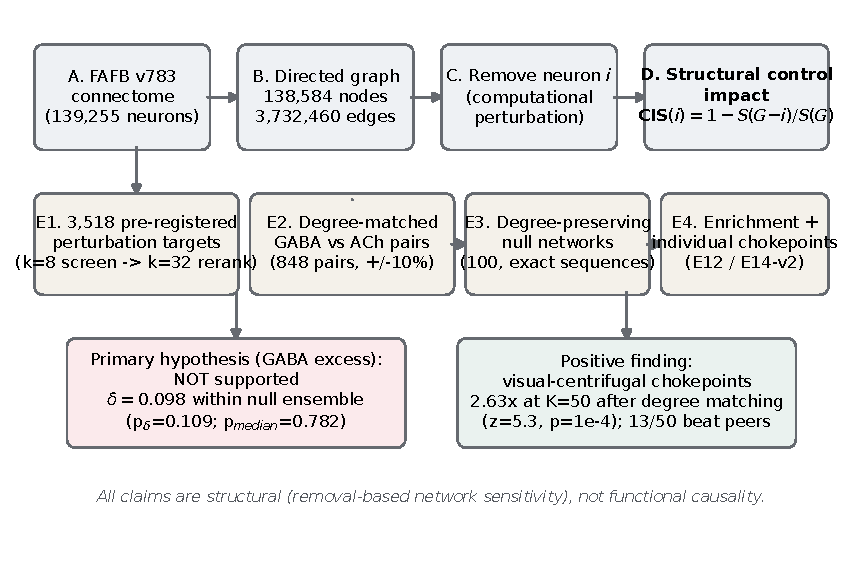
\includegraphics[width=0.95\textwidth]{Figure1}
\caption{\textbf{Study overview.} (A) The FAFB v783 adult female
\emph{Drosophila} connectome (139,255 neurons) is (B) represented as a
binary directed graph (138,584 nodes; 3,732,460 edges). (C) Each
pre-registered target neuron is removed computationally and (D) its
structural control impact is quantified as
$\mathrm{CIS}(i)=1-S(G-i)/S(G)$, the fractional loss of global directed
efficiency. (E) Workflow: 3,518 pre-registered targets screened at $k=8$
and re-ranked at $k=32$; 848 degree-matched GABA--ACh pairs; 100
degree-preserving null networks (exact in/out degree sequences, verified
per null); enrichment and per-node chokepoint analyses. Outcomes: the
GABA-excess hypothesis is not supported ($\delta=0.098$ inside the null
ensemble, $p_\delta=0.109$, $p_{\mathrm{median}}=0.782$), while
visual-centrifugal chokepoints are enriched (2.63$\times$ at $K=50$ after
degree matching, $z=5.3$, $p=10^{-4}$; 13/50 beat degree-matched peers).
All claims are structural (removal-based network sensitivity), not
functional causality.}
\label{fig:overview}
\end{figure}

\begin{figure}[htbp]
\centering
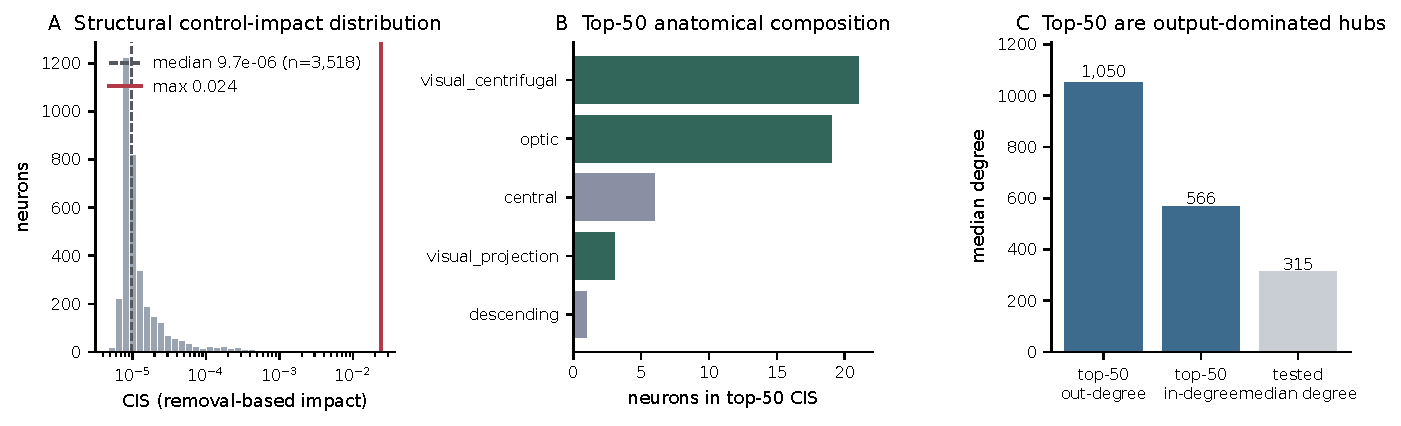
\includegraphics[width=\textwidth]{Figure2}
\caption{\textbf{Network and structural control-impact characterization.}
(A) CIS distribution across the 3,518 pre-registered perturbation targets
(log scale); dashed line: median $9.7\times10^{-6}$; red line: maximum
0.024. (B) Anatomical composition of the top-50 chokepoints by
super-class (green: visual centrifugal/optic; grey: central and other).
(C) Median degrees: top-50 out-degree 1,050 and in-degree 566 versus
tested-population median total degree 315 --- top chokepoints are
output-dominated hubs. $n$: 3,518 (A); 50 (B); medians from the frozen
E13 outputs (C).}
\label{fig:network}
\end{figure}

\begin{figure}[htbp]
\centering
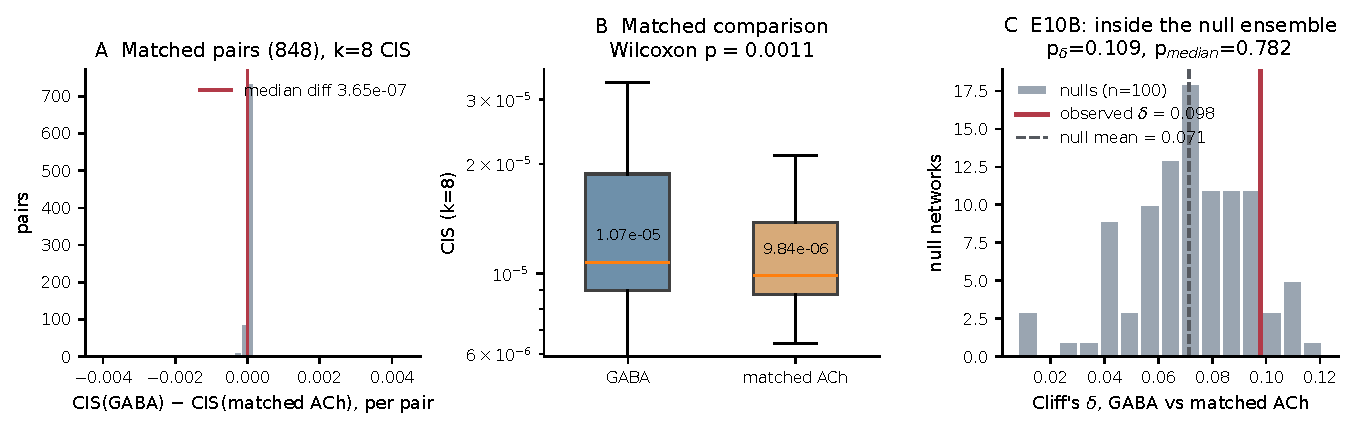
\includegraphics[width=\textwidth]{Figure3}
\caption{\textbf{The GABAergic hypothesis is not supported.}
(A) Per-pair CIS differences (GABA $-$ matched ACh; 848 pairs, $k=8$
screening CIS); red line: median difference $8.7\times10^{-7}$.
(B) Matched CIS distributions (box plots, outliers suppressed; medians
annotated); Wilcoxon $p=0.0011$ reflects the small raw advantage.
(C) The decisive comparison: observed Cliff's $\delta=0.098$ ($k=4$
panel, matched estimator) against the 100-null degree-preserving
ensemble (mean 0.071, sd 0.022); empirical $p_\delta=0.109$,
$p_{\mathrm{median}}=0.782$ --- the observed statistic lies inside the
null ensemble. The visual pairing of (B) and (C) is intentional: a
statistically detectable raw difference can still be fully compatible
with degree-preserving structure.}
\label{fig:gaba}
\end{figure}

\begin{figure}[htbp]
\centering
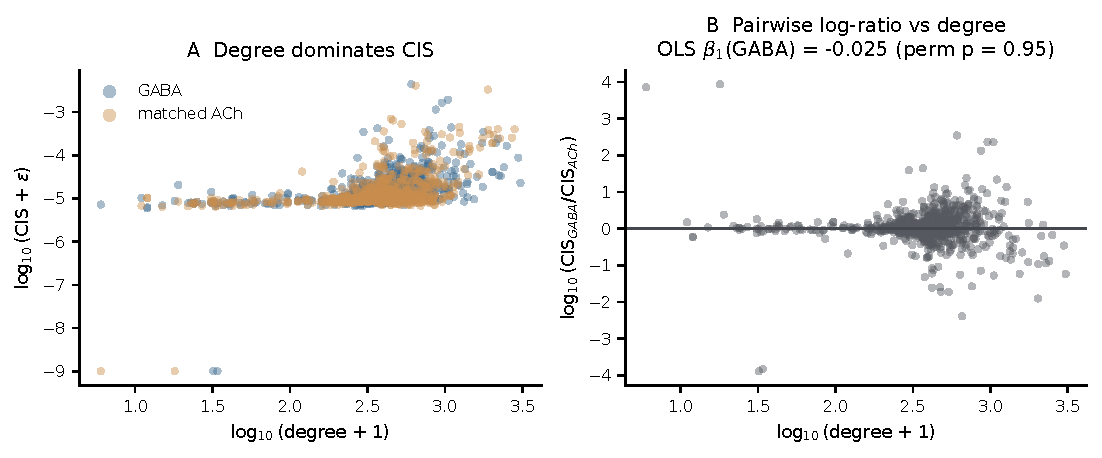
\includegraphics[width=0.85\textwidth]{Figure4}
\caption{\textbf{Degree control.} (A) $\log_{10}$(CIS) versus
$\log_{10}$(degree) for GABA neurons and their matched ACh controls
(848 pairs); CIS rises steeply with degree. (B) Pairwise log-ratio
$\log_{10}(\mathrm{CIS}_{\mathrm{GABA}}/\mathrm{CIS}_{\mathrm{ACh}})$
versus degree; the degree-controlled OLS coefficient for GABA identity is
$\beta_1=-0.025$ (permutation $p=0.95$) --- no residual GABA association
after degree adjustment.}
\label{fig:degctrl}
\end{figure}

\begin{figure}[htbp]
\centering
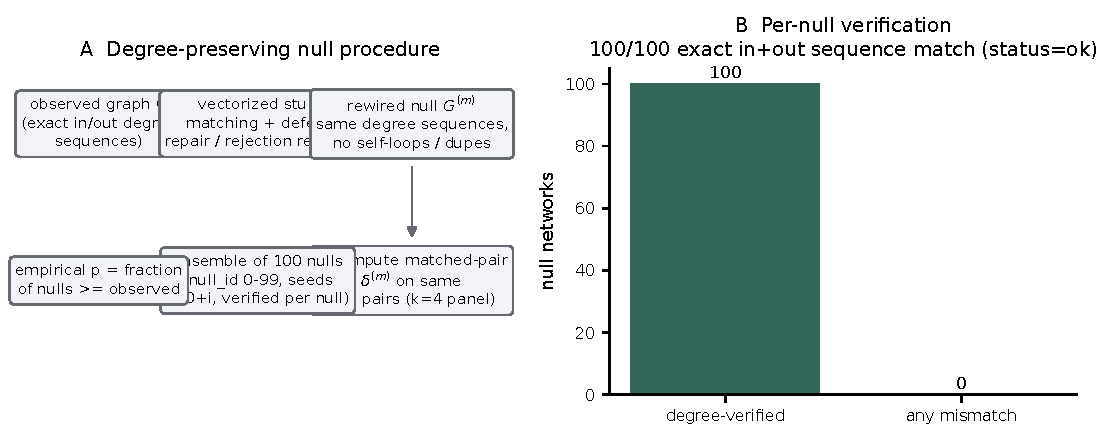
\includegraphics[width=0.85\textwidth]{Figure5}
\caption{\textbf{Degree-preserving null-network framework.} (A) Procedure:
the observed graph is rewired by vectorized stub matching with defect
repair (partner sets distinct from and disjoint to defects) and rejection
redraw; every accepted null preserves both degree sequences exactly and
carries no self-loops or duplicate directed edges; the matched-pair
statistic is recomputed on the same 848 pairs at the same panel size
($k=4$); the ensemble comprises 100 nulls (null\_id 0--99, seeds
$100+i$). (B) Per-null verification: 100/100 nulls show exact in- and
out-degree sequence matches (status ok).}
\label{fig:nullproc}
\end{figure}

\begin{figure}[htbp]
\centering
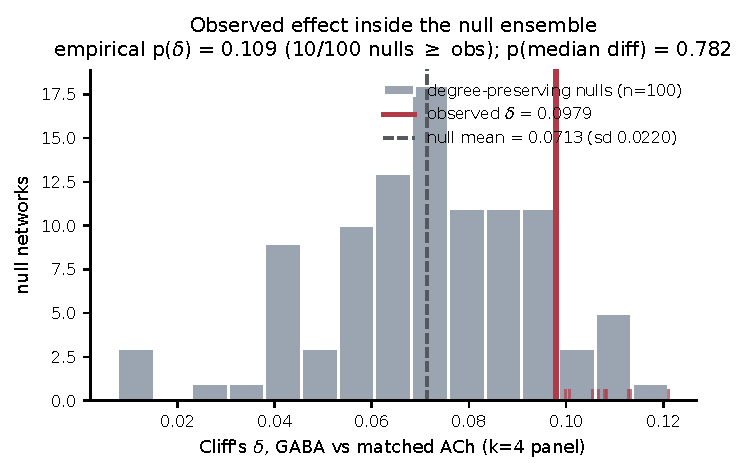
\includegraphics[width=0.7\textwidth]{Figure6}
\caption{\textbf{E10B final null distribution (decisive result).} Grey:
Cliff's $\delta$ for the 100 degree-preserving nulls; red line: observed
$\delta=0.098$; dashed line: null mean $0.071$ (sd 0.022). Red ticks mark
the 10 nulls meeting or exceeding the observation (empirical
$p_\delta=0.109$); the median-difference statistic independently gives
$p=0.782$. The observation lies inside the ensemble: no visual or
statistical excess over degree-preserving structure is implied.
$n=100$ nulls; estimator matched between observation and nulls.}
\label{fig:nulls}
\end{figure}

\begin{figure}[htbp]
\centering
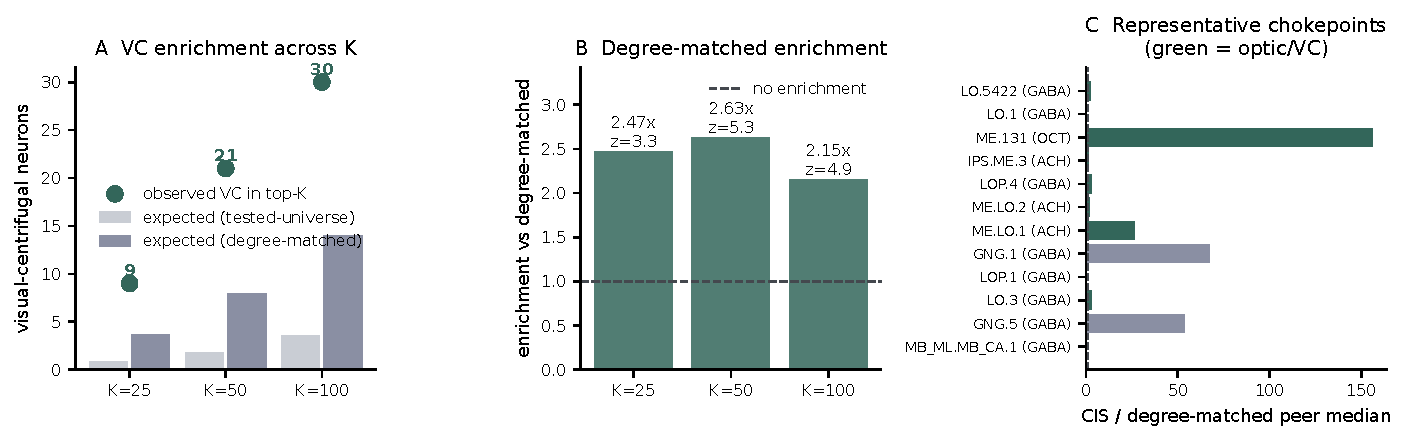
\includegraphics[width=\textwidth]{Figure7}
\caption{\textbf{Visual-centrifugal chokepoints.} (A) Observed
visual-centrifugal counts in the top-$K$ sets (green points) versus
expectations under tested-universe random draws (control A) and
per-slot degree-matched draws (control B), $K=25/50/100$.
(B) Degree-matched enrichment ratios with $z$ scores: 2.47$\times$
($z=3.3$), 2.63$\times$ ($z=5.3$), 2.15$\times$ ($z=4.9$); $p=10^{-4}$
at $K=50$ (10,000 replicates). (C) Representative top-12 chokepoints:
CIS relative to degree-matched peer median (green: optic/visual
centrifugal; grey: other classes); the rank-3 octopaminergic centrifugal
neuron reaches ${\sim}156\times$ its peer median --- a low-degree
structural chokepoint. All identifications are structural; class labels
from Schlegel et al.\ (2024) annotations.}
\label{fig:vc}
\end{figure}

\clearpage
\begin{table}[htbp]
\centering
\small
\caption{\textbf{Dataset and network characteristics.} FlyWire FAFB v783 (Princeton exports); binary directed graph after pair-collapse of the thresholded connection table. All values from the authoritative result files (\texttt{e18\_manifest.json}, E01/E02 outputs).}\label{tab:network}
\begin{tabular}{lr}
\hline
\textbf{Quantity} & \textbf{Value} \\
\hline
Metadata universe (neurons merged) & 139,255 \\
Graph nodes (edge-table universe) & 138,584 \\
Graph edges (collapsed pairs) & 3,732,460 \\
Mean degree & 26.8 \\
Density & $1.92\times10^{-4}$ \\
Reciprocity & 0.083 \\
Largest weak component & 98.4\% \\
Weak components & 875 \\
Pre-registered perturbation targets & 3,518 \\
Degree-matched GABA--ACh pairs & 848 \\
Degree-preserving null networks & 100 (all verified) \\
\hline
\end{tabular}
\end{table}

\begin{table}[htbp]
\centering
\small
\caption{\textbf{Primary GABA hypothesis statistics.} The raw matched-pair effect is small and does not survive degree control (OLS $\beta_1\approx 0$); see Table~\ref{tab:nulls} for the decisive null-ensemble comparison. Source: \texttt{e09\_results.json}.}\label{tab:gaba}
\begin{tabular}{lr}
\hline
\textbf{Statistic} & \textbf{Value} \\
\hline
Matched pairs (GABA vs ACh, total degree $\pm10\%$) & 848 \\
Median difference in CIS (k=8 screening) & 8.75e-07 \\
Cliff's $\delta$ (matched) & 0.111 \\
Wilcoxon signed-rank $p$ & 0.0011 \\
Permutation $p$ (median difference) & 1.0e-04 \\
OLS $\beta_1$ (GABA), $\log_{10}$CIS $\sim$ GABA + $\log_{10}$degree & -0.025 \\
Permutation $p$ on $\beta_1$ (one-sided) & 0.95 \\
Unmatched medians (GABA / ACh) & 1.01e-05 / 9.26e-06 \\
\hline
\end{tabular}
\end{table}

\begin{table}[htbp]
\centering
\small
\caption{\textbf{E10B degree-preserving null-network results.} Every null was verified to preserve both degree sequences exactly before its statistic was admitted. The observed statistic lies inside the null ensemble: the pre-registered hypothesis is rejected (Scenario B). Source: \texttt{results/final/e10b\_final.json} and \texttt{e10b\_nulls.csv}.}\label{tab:nulls}
\begin{tabular}{lr}
\hline
\textbf{Statistic} & \textbf{Value} \\
\hline
Null networks (exact in/out degree preservation) & 100 \\
Observed $\delta$ (k=4 panel, matched estimator) & 0.0979 \\
Null $\delta$: mean $\pm$ sd & 0.0713 $\pm$ 0.0220 \\
Null $\delta$: median / min / max & 0.0729 / 0.0078 / 0.1211 \\
Null $\delta$: 2.5\% / 97.5\% percentile & 0.0193 / 0.1107 \\
Nulls $\geq$ observed & 10 / 100 \\
Empirical $p(\delta)$ & 0.109 \\
Observed median difference & 6.62e-07 \\
Null median-difference mean & 1.53e-06 \\
Empirical $p$(median difference) & 0.782 \\
$z$ vs null ensemble & 1.21 \\
\hline
\end{tabular}
\end{table}

\begin{table}[htbp]
\centering
\small
\caption{\textbf{Visual-centrifugal enrichment of top-K structural chokepoints.} Obs = observed visual-centrifugal count; Exp$_{\mathrm{univ}}$ = expectation under tested-universe random draws (control A); Exp$_{\mathrm{deg}}$ = expectation under per-slot degree-matched draws (control B); Enrichment and $z$ are given against control B, the degree-matched null. Source: \texttt{e12\_strong\_results.json}.}\label{tab:vc}
\begin{tabular}{lrrrrrr}
\hline
K & Obs & Exp$_{\mathrm{univ}}$ & Exp$_{\mathrm{deg}}$ & Enrich. & $z$ & $p$ \\
\hline
K=25 & 9 & 0.9 & 3.6 & 2.47$\times$ & 3.3 & 2.1e-03 \\
K=50 & 21 & 1.8 & 8.0 & 2.63$\times$ & 5.3 & 1.0e-04 \\
K=100 & 30 & 3.6 & 14.0 & 2.15$\times$ & 4.9 & 1.0e-04 \\
\hline
\end{tabular}
\end{table}

\begin{table}[htbp]
\centering
\small
\caption{\textbf{Representative structural chokepoints (E14-v2, selection-bias-corrected).} ``vs peers'' = CIS relative to the median of degree-matched peers (self excluded); emp $p$ = empirical p-value against those peers. NT = predicted neurotransmitter (Schlegel et al. 2024 annotations); all claims are structural, not functional. Source: \texttt{e14\_chokepoint\_catalogue\_v2.csv}.}\label{tab:chokepoints}
\begin{tabular}{rllrrrrl}
\hline
Rank & Neuron & NT & Class & Degree & CIS & vs peers & emp $p$ \\
\hline
1 & LO.5422 & GABA & optic & 12,444 & 2.40\% & 2.4$\times$ & $<$0.0005 \\
2 & LO.1 & GABA & optic & 12,784 & 1.02\% & 0.4$\times$ & 1.000 \\
3 & ME.131 & OCT & visual\_centrifugal & 858 & 0.32\% & 155.9$\times$ & $<$0.0005 \\
4 & IPS.ME.3 & ACH & visual\_centrifugal & 2,063 & 0.03\% & 1.5$\times$ & 0.291 \\
5 & LOP.4 & GABA & optic & 4,021 & 0.04\% & 3.0$\times$ & $<$0.0005 \\
6 & ME.LO.2 & ACH & optic & 1,909 & 0.04\% & 2.0$\times$ & 0.069 \\
7 & ME.LO.1 & ACH & optic & 1,891 & 0.33\% & 26.7$\times$ & $<$0.0005 \\
8 & GNG.1 & GABA & central & 958 & 0.16\% & 67.4$\times$ & 0.024 \\
\hline
\end{tabular}
\end{table}


\section*{Data and code availability}
Data: FlyWire FAFB v783 (Princeton exports), CC BY-NC 4.0 --- cite
Dorkenwald et al.\ (2024), Schlegel et al.\ (2024), Matsliah et al.\
(2024). Code: repository \texttt{src/}, \texttt{tests/}, and
\texttt{scripts/}; full manifest \texttt{results/tables/e18\_manifest.json};
deliverable hashes \texttt{dist/SHA256SUMS.txt}.

\bibliographystyle{unsrt}
\bibliography{references}

\end{document}
